\section{Driver Interface Module}

The driver interface module implements the design specified in Sec.\ \ref{sec:Driver-Interface-Module}. The hardware and software aspects of this module's implementation are discussed in this section. Figure \ref{fig:driver_interface_pcb} shows a photo of the completely populated and debugged driver interface module hardware.

\begin{figure}[h]
\centering
\includegraphics[scale=1]{implementation/figures/driver_interface_pcb.eps}
\caption{Populated telemetry module PCB.}\label{fig:driver_interface_pcb}
\end{figure}

\subsection{Hardware}

In addition to the base system hardware common to all modules described in Sec.\ \ref{sec:base_system_hardware}, the driver interface module provides all of the support hardware needed for the LCD module to function. An FPC connector, LCD bias boost converter, \unit{+3.3}{\volt} power supply, latch for the interface to the microcontroller, as well as level translators to translate from the microcontroller's \unit{+5}{\volt} logic to the LCD Controller's \unit{+3.3}{\volt} logic are all included in the module. Additionally, 3 rotary encoders are soldered on the board. On the back of the PCB are connectors to the steering wheel-mounted push buttons and paddles.

The LCD module used in the driver interface implementation is a packaged LCD module from Newhaven Display. Along with the actual LCD panel, a built-in display controller chip and display RAM are included. Interfacing with the LCD module entails interfacing with it's controller chip, a SED1335 LCD controller IC from Seiko Epson Corporation. The controller chip handles all of the low level functionality of the LCD, such as generating pixel clocks and drawing to the screen from the LCD RAM. It also provides a character generator.

\subsubsection{LCD Module Bias Circuit}

According to the datasheet, the LCD screen requires a large bias voltage of \unit{+22}{\volt} \cite{LCD_Module}. A Linear Technology LT1615 step-up DC/DC converter was chosen as the centre of a boost converter circuit to generate the bias voltage, shown in Fig.\ \ref{fig:lcd_boost_converter}.

\begin{figure}[htp]
 \centering
 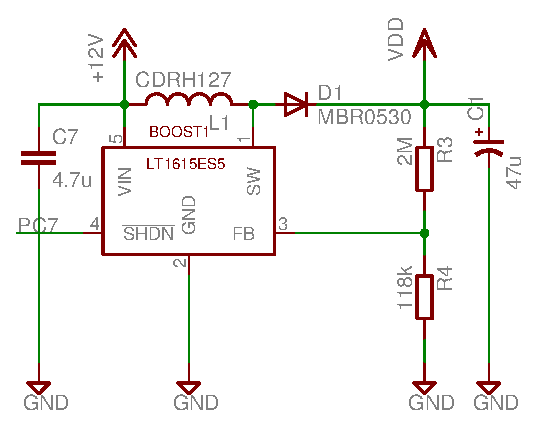
\includegraphics[scale=0.8]{implementation/figures/driver_interface_lcd_bias_circuit.eps}
 \caption{Boost converter circuit}
 \label{fig:lcd_boost_converter}
\end{figure}

\paragraph{Inductor Selection}

According to the datasheet, the value of the inductor $L_1$ can be determined by the following equation:

\begin{equation}
L_1=\frac{V_{out}-V_{in(min)}+V_{D}}{I_{limit}}\cdot t_{off}\label{IndSel}
\end{equation}

Where $V_D$ is the diode D1's forward voltage drop, $V_{out}$ the desired output voltage of the converter, $V_{in(min)}$ the minimum expected suppy voltage, and $I_{limit}$ the switching current limit of the converter device, between \unit{300}{\milli\ampere} and \unit{400}{\milli\ampere}, and $t_{off}$ the switching off-time of the converter device, typically \unit{400}{\nano\second}.

Using (\ref{IndSel}) with $V_{D}=\unit{0.4}{\volt}$, $I_{limit}=\unit{350}{\milli\ampere}$, $t_{off}=\unit{400}{\nano\second}$, $V_{out}=+\unit{22}{\volt}$, and $V_{in(min)}=\unit{11.5}{\volt}$ gives $L\approx\unit{12.45}{\micro\henry}$. The datasheet however suggests a value slightly smaller than calculated should be suitable with only slight decrease in maximum output current. Since the LCD requires very little current (estimated less than \unit{1}{\milli\ampere}, we used an inductor value of $\unit{10}{\micro\henry}$.


\paragraph{Output Voltage}

To obtain a $V_{bias}$ of $+\unit{22}{\volt}$, two resistors in the bias circuit provide a voltage divided feedback path from the output to the FB pin on the LT1615. The eqation relating the output voltage with the resistor values is

\begin{equation}
R_{3}=R_{4}\cdot\left(\frac{V_{bias}}{1.23}-1\right)
\end{equation}

 $R_{3}$ was chosen to be $\unit{2}{\mega\ohm}$ to limit current flowing from the output to ground, and a suitable $R_{4}$ of $\unit{118}{\kilo\ohm}$ was found.


\subsubsection{LCD Module Data Interface\label{sec:lcd_module_data_interface}}

The LCD's 8-bit interface was suitable to be connected to the AT90CAN128's external memory interface. This way the LCD becomes a memory-mapped periferal to the microcontroller, and all the control signals (Read and Write strobes, etc.), are handled by the memory controller.

The AT90CAN128's external memory interface uses Port A pins 0-7 as a multiplexed data and address bus which must be demultiplexed in order to offer seperate address and data busses. In operation, the external memory interface first puts out the address on the combined bus, followed by the data. The ALE (Address Latch Enable) signal signifies the difference \cite{AT90CAN}.

In order to provide seperate address and data busses for the LCD controller, a fast octal D-Type latch from NXP was chosen to latch the address from the AT90CAN128. The width of the ALE pulse, $t_{LHLL}$, provided by the AT90, is specified in the datasheet as

\nomenclature{$t_{LHLL}$}{The Address Latch Enable pulse width on the AT90CAN128's external memory interface}

\begin{equation}
t_{LHLL}=t_{CLCL}-15\, \nano\second
\end{equation}

where $t_{CLCL}$ is the main clock period. With the main clock running at $\unit{16}{\mega\hertz}$, $t_{LHLL}=\unit{48}{\nano\second}$.

\nomenclature{$t_{CLCL}$}{The main system clock period on the AT90CAN128.}

The 74LVC373A latch from NXP requires a minimum LE pulse width of $\unit{4.5}{\nano\second}$, so is suitable as a demultiplexing interface.

The external memory on the AT90CAN128 starts at address 0x1100h, and there are two possible registers to read/write to on the LCD controller. The LCD controller therefore has it's single address select pin connected to the LSB of the address lines output from the latch. Since only two addresses are required, the upper 8 address lines of the external memory interface were not used.

A logical combination of the lower byte address lines should be connected to the CS (Chip Select) line on the LCD controller. Since the external memory controller only outputs control signals when the requested memory operation is in external space, it is safe to ignore the upper byte address lines.

\nomenclature{CS}{Chip Select}

It was chosen to tie the 2nd bit of the address lines to CS. The resulting operations when interacting with the LCD controller are summarized in Table \ref{tab:lcd_memory_map}.

\begin{table}
\caption{Memory-mapped LCD Interface}
\label{tab:lcd_memory_map}
\centering{}
\begin{tabular}{|l|l|l|}
\hline 
Address  & Read Function  & Write Function\tabularnewline
\hline
\hline 
0x1101  & Status flag read  & Display data and parameter write\tabularnewline
\hline 
0x1102  & Display dada and cursor address read  & Command write\tabularnewline
\hline
\end{tabular}
\end{table}

\subsection{Software}

The system software running on the Telemetry module acts as a source of commands to the other modules on the network, and serves to meet the design outlined in Sec.\ \ref{sec:Driver-Interface-Module}. The majority of the software implemented is in support of the LCD hardware. The software supporting the buttons, knobs, and paddles is in comparison very simple.

\subsubsection{LCD Module Library}

An LCD module library was written to implement the entire command set of the SED1335. The functionality covers initializing the LCD Controller and screen from reset as well as setting up different layers and cursors, and drawing strings and bitmaps. Additionally, more complex drawing operations were implemented specifically to meet the requirements of the driver interface module, such as progress bars, underlines, a clock at the top of the screen, and the signal strength indicator. The parameter menu system was also implemented that allows the driver to scroll through the list of vehicle parameters to tune.

\subsubsection{Font Loading\label{sec:lcd_module_font_loading}}

The built-in font in the SED1335 LCD controller is only 5x7 pixels, and difficult to read. To display more readable text on the LCD screen, a custom 16x16 pixel fixed-width font for the character generator was developed in a series of steps:
\begin{enumerate}
 \item a 43 character subset of standard ASCII was chosen to be implemented, the capital letters A-Z, the numbers, and a few punctuation characters;
 \item next, a 688x16 pixel image was created in The Gimp image manipulation program. 16 pixel wide blocks were sectioned off, and using The Gimp's text tool, fixed width characters were drawn on the image at 16 pixel intervals;
  \item then, using The Gimp's python scripting interface, a small python script was written to pull the bitmap data out of the image and format it in such a way as could be placed in a standard c include file as a \emph{const char} array.
\end{enumerate}

A library was written for the driver interface module that at runtime loads this constant font data into the appropriate character generator ram on the LCD. Now, ASCII characters written to the character buffer in the LCD memory are drawn by the character generator and show up on the screen in the custom font. An image of the font used is shown in Fig.\ \ref{fig:driver_interface_font}.

\begin{figure}[htp]
 \centering
 
\includegraphics[scale=1]{implementation/figures/driver_interface_font.eps}
 \caption{Custom 16x16 pixel fixed-width font.}
 \label{fig:driver_interface_font}
\end{figure}

\subsubsection{I/O Library}

A small I/O Library was written to set up and manage the interrupts generated by the buttons, knobs, and paddles on the steering wheel.
 
%\subsubsection{Vehicle Diagnostics Library}
% 
% 
%\subsubsection{Vehicle Parameter Library}
% 
% 
% \subsubsection{Vehicle Dynamic Mode}


\subsubsection{CAN Interface}

A CAN Interface library was written to interface the rest of the driver interface module system software with events happening on the network. In particular, the CAN Interface library sends out upshift and downshift requests to the Transmission module when the I/O library indicates that a paddle has been pulled. The start and neutral find buttons operate in the same fashion. The driver interface module receives incoming dashboard data from the other modules, such as vehicle wheel speed, and Telemetry signal strength.

\subsubsection{Main Control Loop}